\newpage
\subsection{Caso d'uso UC 4: Applicazione demo lista-spesa.}
\label{Caso d'uso UC 4: Applicazione demo lista-spesa.}
\begin{figure}[ht]
	\centering
	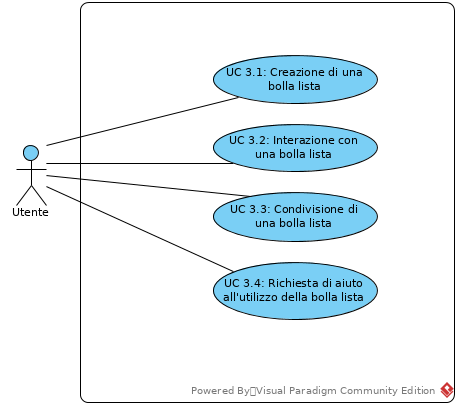
\includegraphics[scale=0.60]{Usecases/img/UC4.png}
	\caption{Caso d'uso UC 4: Applicazione demo lista spesa.}
\end{figure}


\FloatBarrier
\begin{itemize}
\item \textbf{Attori:} Utente.
\item \textbf{Descrizione:} L'utente utilizza l'applicazione demo lista-spesa.
\item \textbf{Precondizione:} L'utente vuole utilizzare l'applicazione demo lista-spesa. 
\item \textbf{Postcondizione:} L'utente ha utilizzato l'applicazione demo lista-spesa.
\item \textbf{Scenario principale:}
	\begin{itemize}
	\item{Creazione di una bolla lista-spesa (UC 4.1).}
	\item{Interazione con una bolla lista-spesa (UC 4.2).}
	\item{Condivisione di una bolla lista-spesa (UC 4.3).}
	\item{Richiesta di aiuto all'utilizzo della bolla lista spesa (UC 4.4).}
	\end{itemize}

\end{itemize}